\documentclass{standalone}
\usepackage{tikz-feynman}

\begin{document}

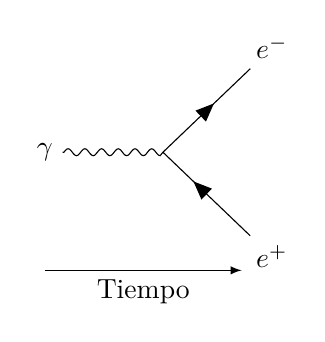
\begin{tikzpicture}
  \begin{feynman}
    % Definir los vértices
    \vertex (a) {\(\gamma\)};
    \vertex [right=of a] (b);
    \vertex [above right=of b] (f1) {\(e^{-}\)};
    \vertex [below right=of b] (c) {\(e^{+}\)};

    % Dibujar el diagrama
    \diagram* {
      (a) -- [boson] (b) -- [fermion] (f1),
      (b) -- [anti fermion] (c),
    };

    % Dibujar la flecha del tiempo
    \draw[-latex] (0,-1.5) --(2.5, -1.5) node[midway, below] {Tiempo};
  \end{feynman}
\end{tikzpicture}

\end{document}
